\documentclass[a4paper]{article}
%\usepackage{a4wide}
\usepackage{fullpage}
\usepackage[metapost,mplabels,truebbox]{mfpic}
\usepackage[pdftex]{graphicx}
\usepackage{hyperref}
\graphicspath{{pics/}{mfpics/}}
\usepackage{amsmath,amssymb,amsthm}
\usepackage{verbatim}
\usepackage{tikz}

\newcommand{\N}         {{\mathbb{N}}}
\newcommand{\Z}         {{\mathbb{Z}}}
\newcommand{\Q}         {{\mathbb{Q}}}
\newcommand{\R}         {{\mathbb{R}}}
\newcommand{\C}         {{\mathbb{C}}}
\newcommand{\bbm}       {\begin{bmatrix}}
\newcommand{\bsm}       {\left[\begin{smallmatrix}}
\newcommand{\ebm}       {\end{bmatrix}}
\newcommand{\esm}       {\end{smallmatrix}\right]}
\newcommand{\bcf}[2]{\left(\begin{array}{c}{#1}\\{#2}\end{array}\right)}
\newcommand{\tm}        {\times}
\newcommand{\iffa}      {\Leftrightarrow}
\newcommand{\ip}[1]     {\langle #1\rangle}

\newcommand{\CH}        {\mathcal{H}}
\newcommand{\CM}        {\mathcal{M}}

\newcommand{\al}        {\alpha}
\newcommand{\bt}        {\beta}
\newcommand{\gm}        {\gamma}
\newcommand{\dl}        {\delta}
\newcommand{\ep}        {\epsilon}
\newcommand{\zt}        {\zeta}
\newcommand{\et}        {\eta}
\newcommand{\tht}       {\theta}
\newcommand{\io}        {\iota}
\newcommand{\kp}        {\kappa}
\newcommand{\lm}        {\lambda}
\newcommand{\ph}        {\phi}
\newcommand{\ch}        {\chi}
\newcommand{\ps}        {\psi}
\newcommand{\rh}        {\rho}
\newcommand{\sg}        {\sigma}
\newcommand{\om}        {\omega}

\newcommand{\vph}       {\varphi}

\newcommand{\Sg}        {\Sigma}
\newcommand{\Dl}        {\Delta}
\newcommand{\sm}        {\setminus}
\newcommand{\sse}       {\subseteq}
\newcommand{\st}        {\;|\;}
\newcommand{\xra}       {\xrightarrow}
\newcommand{\ov}        {\overline}

\newcommand{\rr}        {\sqrt{3}}
\newcommand{\rs}        {\sqrt{6}}
\newcommand{\rt}        {\sqrt{2}}


\newcommand{\half}      {{\textstyle\frac{1}{2}}}

\renewcommand{\:}{\colon}



\newcounter{probcounter}
\newcounter{marksassigned}
\newcounter{marksawarded}
\newcounter{totalmarks}

\newcommand{\mrks}[1]{%
\addtocounter{marksassigned}{#1}%
\addtocounter{totalmarks}{#1}%
\textbf{(#1 marks)}}
\newcommand{\mks}[1]{\addtocounter{marksawarded}{#1}\textbf{\color{red}[#1]}}
\newcommand{\mk}{\mks{1}}

\newenvironment{problem}{
\stepcounter{probcounter}
\setcounter{marksawarded}{0}
\bigskip\par\noindent\hypertarget{Q\roman{probcounter}}{\textbf{(\arabic{probcounter})}}
}{
\typeout{Q\arabic{probcounter}: \arabic{marksassigned} marks assigned}
\setcounter{marksassigned}{0}
}

\newenvironment{solution}{
{\bigskip\par\noindent \bf Solution:}}{
%\newpage
\typeout{Q\arabic{probcounter}: \arabic{marksawarded} marks awarded}
}

\newcommand{\printtotalmarks}{%
\typeout{Total assigned: \arabic{totalmarks} marks}%
}

\newcommand{\sct}{\section}




\begin{document}

\begin{center}
 {\Huge Galois theory --- All exam questions}
\end{center}
\vspace{4ex}

\begin{problem}% 0910 Q1
 Put $L=\Q(\sqrt{7},\sqrt{13})$ and $\al=\sqrt{7}+\sqrt{13}\in L$.
 \begin{itemize}
  \item[(a)] Give a basis for $L$ over $\Q$. \mrks{2}
  \item[(b)] Define the Galois group $G(L/\Q)$, and list all its
   elements. \mrks{3}  
  \item[(c)] Let $\al_0,\dotsc,\al_r$ be the images of $\al$ under all
   the automorphisms of $L$.  Calculate the sum $\al_0+\dotsb+\al_r$
   and the product $\al_0\al_1\dotsb\al_r$. \mrks{4}
  \item[(d)] Find a monic polynomial $f(x)$ of degree four over $\Q$
   such that $f(\al)=0$.  \mrks{3}
  \item[(e)] Consider an element
   $a=w+x\sqrt{7}+y\sqrt{13}+z\sqrt{91}\in L$, and suppose that
   $a^2\in\Q$.  By considering the action of automorphisms on $a$ and
   $a^2$, prove that 
   \[ a\in \Q\;\cup\; \Q.\sqrt{7} \;\cup\; \Q.\sqrt{13} \;\cup\; \Q.\sqrt{91}.
   \]
   \mrks{7}
  \item[(f)] Describe all the subfields $K$ with $\Q\sse K\sse L$,
   justifying your answer briefly.  For each such field $K$, state the
   values of $[L:K]$ and $[K:\Q]$. \mrks{6}
 \end{itemize}
\end{problem}
\begin{solution}
 \textbf{Parts~(a), (b), (d) and (f) are standard, and very similar to
 examples in the notes and exercises.  Part~(c) will not be familiar
 but nonetheless is easy.  Part~(e) is intended to be more challenging.}
 \begin{itemize}
  \item[(a)] The list $1,\sqrt{7},\sqrt{13},\sqrt{7}\sqrt{13}$ is a
   basis for $L$ over $\Q$. \mks{2}
  \item[(b)] $G(L/\Q)$ is the group of automorphisms of $L$ (that act
   as the identity on $\Q$). \mk There are four such automorphisms, as
   follows: 
   \begin{align*}
    \sg_0(w+x\sqrt{7}+y\sqrt{13}+z\sqrt{7}\sqrt{13}) &= 
      w+x\sqrt{7}+y\sqrt{13}+z\sqrt{7}\sqrt{13} \\
    \sg_1(w+x\sqrt{7}+y\sqrt{13}+z\sqrt{7}\sqrt{13}) &= 
      w-x\sqrt{7}+y\sqrt{13}-z\sqrt{7}\sqrt{13} \\
    \sg_2(w+x\sqrt{7}+y\sqrt{13}+z\sqrt{7}\sqrt{13}) &= 
      w+x\sqrt{7}-y\sqrt{13}-z\sqrt{7}\sqrt{13} \\
    \sg_3(w+x\sqrt{7}+y\sqrt{13}+z\sqrt{7}\sqrt{13}) &= 
      w-x\sqrt{7}-y\sqrt{13}+z\sqrt{7}\sqrt{13}.  \mks{2}
   \end{align*}
  \item[(c)] The relevant images are 
   \begin{align*}
    \al_0 &= +\sqrt{7}+\sqrt{13} & \al_1 &= -\sqrt{7}+\sqrt{13} \\
    \al_2 &= +\sqrt{7}-\sqrt{13} & \al_3 &= -\sqrt{7}-\sqrt{13}. \mk
   \end{align*}
   From this it is clear that $\al_0+\al_1+\al_2+\al_3=0$ \mk.  We also
   have $\al_0\al_1=(\sqrt{7})^2-(\sqrt{13})^2=7-13=-6$ and similarly
   $\al_2\al_3=-6$ so $\al_0\al_1\al_2\al_3=36$. \mks{2}
  \item[(d)] We have $\al^2=7+2\sqrt{7}\sqrt{13}+13=20+2\sqrt{91}$ \mk, so
   $(\al^2-20)^2=4\tm 91=364$ \mk.  Thus, if we put
   $f(x)=(x^2-20)^2-364=x^4-40x^2+36$ then $f(\al)=0$ \mk.
  \item[(e)] Consider an element
   $a=w+x\sqrt{7}+y\sqrt{13}+z\sqrt{91}\in K$ with $a^2\in\Q$.  For
   any automorphism $\sg_i$, we then have $\sg_i(a)^2=\sg_i(a^2)=a^2$,
   so $\sg_i(a)=\pm a$ \mks{2}.  Recall that 
   \[ \sg_1(a) = w-x\sqrt{7}+y\sqrt{13}-z\sqrt{7}\sqrt{13}. \]
   This is only equal to $a$ if $x=z=0$, and is only equal to $-a$ if
   $w=y=0$ \mk.  From this and the parallel arguments for $\sg_2$ and
   $\sg_3$, we see that 
   \begin{itemize}
    \item[(1)] either $w=y=0$, or $x=z=0$;
    \item[(2)] either $w=x=0$, or $y=z=0$;
    \item[(3)] either $w=z=0$, or $x=y=0$. \mks{2}
   \end{itemize}
   Suppose that $w\neq 0$; then we see from~(1) that $x=z=0$, and
   from~(2) that $y=z=0$, so $x=y=z=0$, so $a\in\Q$.  Similarly, if
   $x\neq 0$ we see from~(1) that $w=y=0$, and from~(2) that $y=z=0$,
   so $w=y=z=0$ and $a\in\Q.\sqrt{7}$.  In the same way, if
   $y\neq 0$ then $w=x=z=0$ and $a\in\Q.\sqrt{13}$, and if
   $z\neq 0$ then $w=x=y=0$ and $a\in\Q.\sqrt{91}$. \mks{2}
  \item[(f)] The intermediate fields between $\Q$ and $K$ biject with
   the subgroups of $G(K/\Q)$ \mk.  If we put $H_i=\{\sg_0,\sg_i\}$ then
   the full list of subgroups is $\{1\},H_1,H_2,H_3$ and $G(K/\Q)$
   itself \mks{2}, so the intermediate fields are 
   \begin{align*}
    K^{\{1\}} &= K \\
    K^{H_1} &= \Q(\sqrt{13}) \\
    K^{H_2} &= \Q(\sqrt{7}) \\
    K^{H_3} &= \Q(\sqrt{7}\sqrt{13}) \\
    K^{G(K/\Q)} &= \Q. \mks{2}
   \end{align*}
   The degrees are $[K:\Q]=4$ and $[K:K^{H_i}]=[K^{H_i}:\Q]=2$.  \mk
 \end{itemize}
\end{solution}

\begin{problem}% 1011 Q1
 \begin{itemize}
  \item[(a)] Define what is meant by an \emph{automorphism} of a
    field. \mrks{3}
  \item[(b)] Let $K$ be an extension field of $\Q$, and let $\phi$ be
   an automorphism of $K$.  Prove that $\phi(q)=q$ for all $q\in\Q$.
   \mrks{5}
  \item[(c)] Define the \emph{Galois group} $G(L/K)$ for a field
   extension $K\leq L$. \mrks{2}
  \item[(d)] Show that $G(\Q(i)/\Q)$ is a cyclic group of order two.
   (Your proof should be complete and self-contained, except that you
   may assume part~(b).) \mrks{9}
  \item[(e)] Give an example of an extension $K\leq L$ where $[L:K]=4$
   but $|G(L/K)|=2$.  Justify your answer.
   \mrks{6}
 \end{itemize}
\end{problem}
\begin{solution}
 \begin{itemize}
  \item[(a)] \textbf{(Bookwork)}
   An automorphism of a field $K$ is a bijective \mk map
   $\phi\:K\to K$ such that 
   \begin{itemize}
    \item $\phi(0)=0$ and $\phi(1)=1$. \mk
    \item $\phi(a+b)=\phi(a)+\phi(b)$ for all $a,b\in K$.
    \item $\phi(ab)=\phi(a)\phi(b)$ for all $a,b\in K$. \mk
   \end{itemize}
  \item[(b)] \textbf{(Bookwork)}
   Let $\phi\:K\to K$ be an automorphism, where $\Q\leq K$.
   We first claim that $\phi(n)=n$ for all $n\in\N$.  Indeed, this is
   true for $n=0$ and $n=1$ by the definition of a homomorphism.\mk  If
   $\phi(n)=n$ for some $n$, it follows that
   \[ \phi(n+1)=\phi(n)+\phi(1)=n+1. \mk \]
   We therefore see by induction that $\phi(n)=n$ for all $n\in\N$.
   From this, we see that
   \[ n+\phi(-n)=\phi(n)+\phi(-n)=\phi(n+(-n))=\phi(0)=0, \]
   which gives $\phi(-n)=-n$ for all $n\in\N$, so $\phi(m)=m$ for all
   $m\in\Z$ \mk.  Now suppose that $n,m\in\Z$ with $n>0$, and put
   $q=m/n\in\Q$.  As $nq=m$ and $n,m\in\Z$ we have 
   \[ n\,\phi(q) = \phi(n)\phi(q)=\phi(nq)=\phi(m)=m, \]
   so $\phi(q)=m/n=q$ \mks{2}.  As every element of $\Q$ can be written as
   $m/n$ for some such $m$ and $n$, we deduce that
   $\phi|_{\Q}=1_{\Q}$ as required.
  \item[(c)] \textbf{(Bookwork)}
   $G(L/K)$ is defined to be the set of all automorphisms
   $\tht\:L\to L$ \mk that satisfy $\tht(a)=a$ for all $a\in K$ \mk.
  \item[(d)] \textbf{(This is a rearrangement/specialisation of 
   standard material.)}
   $\Q(i)$ is the set of complex numbers of the form
   $a=x+iy$ with $x,y\in\Q$.  We can define $\sg\:\Q(i)\to\Q(i)$ by
   $\sg(x+iy)=x-iy$ \mk.  This has $\sg(0)=0$ and
   $\sg(1)=\sg(1+0i)=1-0i=1$.  If $b=u+iv$ (with $u,v\in\Q$) then it
   is clear that $\sg(a+b)=\sg(a)+\sg(b)$ \mk.  We also have
   \begin{align*}
    \sg(ab) &= \sg(xu-yv+(xv+yu)i) = xy-yv-(xv+yu)i \\
     &= (x-iy)(y-iv) = \sg(a)\sg(b). \mk
   \end{align*}
   This proves that $\sg$ is a homomorphism from $\Q(i)$ to $\Q(i)$.
   it is also clear that $\sg^2(a)=\sg(x-iy)=x+iy=a$ for all $a$, so
   $\sg$ is its own inverse, so it is an automorphism \mk.  

   Now let $\tau\:\Q(i)\to\Q(i)$ be an arbitrary automorphism.  Note
   that $\tau(i)^2+1=\tau(i^2+1)=\tau(0)=0$ \mk.  From this it is clear
   that $\tau(i)\in\{i,-i\}$.  Note also that $\tau(x)=x$ for all
   $x\in\Q$ by part~(b) \mk.  Thus, if $\tau(i)=i$ we have
   $\tau(x+iy)=\tau(x)+\tau(i)\tau(y)=x+iy$, so $\tau=1_{\Q(i)}$ \mk.  On
   the other hand, if $\tau(i)=-i$ we have
   $\tau(x+iy)=\tau(x)+\tau(i)\tau(y)=x-iy=\sg(x+iy)$ for all $x$ and
   $y$, so $\tau=\sg$ \mk.  This proves that $G(\Q(i)/\Q)=\{1,\sg\}$,
   which is a cyclic group of order two \mk.
  \item[(e)] \textbf{(Unseen)}
   Take $K=\Q$ and $L=\Q(2^{1/4})\leq\R$ \mks{3}.  As
   $L\simeq\Q[x]/(x^4-2)$ we see that automorphisms of $L$ biject with
   roots of $x^4-2$ in $L$ \mks{2}, of which there are precisely two
   (namely $2^{1/4}$ and $-2^{1/4}$) so $|G(L/K)|=2$ \mk.
 \end{itemize}
\end{solution}

\begin{problem}% 1112 Q1
 \begin{itemize}
  \item[(a)] Explain what is meant by the following. \mrks{7}
   \begin{itemize}
    \item[(1)] A \emph{homomorphism} of fields.
    \item[(2)] The \emph{degree} of a homomorphism.
    \item[(3)] An \emph{automorphism} of a field.
    \item[(4)] The \emph{Galois group} of a field extension.
   \end{itemize}
  \item[(b)] Show that any homomorphism of fields is injective. \mrks{5}
  \item[(c)] Let $N/K$ be a field extension of finite degree.  Explain
   what it means for $N$ to be \emph{normal} over $K$.  You should give
   one criterion in terms of roots of polynomials, and another
   criterion in terms of numbers of homomorphisms. \mrks{5}
  \item[(d)] Which of the following fields are normal over $\Q$?
   Justify your answers briefly. \mrks{8}
   \begin{align*}
    L_1 &= \Q(\sqrt{11},\sqrt{13}) \\
    L_2 &= \Q(e^{2\pi i/11}) \\
    L_3 &= \Q(2^{1/11}) \\
    L_4 &= \Q\left(\sqrt{3+\sqrt{7}}\right)
   \end{align*}
 \end{itemize}
\end{problem}
\begin{solution}
 \begin{itemize}
  \item[(a)] \textbf{Bookwork} 
   \begin{itemize}
    \item[(1)] Let $K$ and $L$ be fields.  A \emph{homomorphism} from
     $K$ to $L$ is a function $\phi\:K\to L$ such that 
     \begin{align*}
      \phi(0_K) &= 0_L \\
      \phi(1_K) &= 1_L \\
      \phi(a+b) &= \phi(a)+\phi(b) & & \text{ for all } a,b\in K \\
      \phi(ab)  &= \phi(a)\phi(b)  & & \text{ for all } a,b\in K. \mks{2}
     \end{align*}
     (The first condition here could be omitted as it follows from the
     third.  However, the second condition does not follow from the
     fourth one, because $\phi$ could be zero.)
    \item[(2)] The \emph{degree} of a homomorphism $\phi$ as above is
     the dimension of $L$ considered as a vector space over the
     subfield $\phi(K)$. \mks{2}
    \item[(3)] An \emph{automorphism} of $K$ is a bijective
     homomorphism from $K$ to itself. \mk
    \item[(4)] Let $L$ be a field extension of $K$.  The \emph{Galois
      group} $G(L/K)$ is the group of all automorphisms $\phi\:L\to L$
     that satisfy $\phi(a)=a$ for all $a\in K$. \mks{2}
   \end{itemize}
  \item[(b)] \textbf{I will give the students a list of 8-10 proofs to
   learn, of which this will be one.}
   Let $\phi\:K\to L$ be a homomorphism of fields.  We first
   claim that if $a\in K$ and $a\neq 0$ then $\phi(a)\neq 0$. \mk Indeed,
   as $a\neq 0$ there exists $b\in K$ with $ab=1$, so
   $\phi(a)\phi(b)=\phi(ab)=\phi(1)=1$.  However, if $\phi(a)$ were
   $0$ we would instead have $\phi(a)\phi(b)=0\tm\phi(b)=0$, which is
   impossible because $0\neq 1$. \mks{2}

   Now suppose we have $u,v\in K$ with $u\neq v$.  This means that
   $u-v\neq 0$, so by the previous paragraph the element
   $\phi(u)-\phi(v)=\phi(u-v)$ is nonzero, so $\phi(u)\neq\phi(v)$.
   Thus, $\phi$ is injective. \mks{2}
  \item[(c)] \textbf{Bookwork}
   Let $N/K$ be a field extension of finite degree.  We say
   that $N$ is \emph{normal} over $K$ if for every monic irreducible
   polynomial $f(x)\in K[x]$, either $f$ has no roots in $N$ or $f$
   splits properly over $N$ \mks{3}.  One can show that this is equivalent to
   the following criterion: for any other extension $L/K$, either
   $E_K(L,N)=\emptyset$ or $|E_K(L,N)|=[L:K]$ (where
   $E_K(L,N)=\{\phi\:L\to N\st \phi|_K=1\}$). \mks{2}  (Alternatively,
   it is equivalent to say that $|G(N/K)|=[N:K]$; two marks will also
   be given for this answer.)
  \item[(d)] \textbf{Similar to examples in the notes and problem sheets.}
   The field $L_1$ is the splitting field for
   $(x^2-11)(x^2-13)$ over $\Q$, \mk so it is normal \mk.  Similarly, $L_2$ is
   the splitting field for $x^{11}-1$ (or for the cyclotomic
   polynomial $\vph_{11}(x)$) \mk and so is normal over $\Q$ \mk.  However,
   $L_3$ contains the unique real root of the polynomial $x^{11}-2$
   but none of the non-real roots (such as $e^{2\pi i/11}2^{1/11}$) \mk,
   so it cannot be normal \mk.  Similarly, $L_4$ contains the number
   $\al=\sqrt{3+\sqrt{7}}$ which is a root of the irreducible
   polynomial $f(x)=(x^2-3)^2-7=x^4-6x^2+2$, but it does not contain the
   number $\bt=\sqrt{3-\sqrt{7}}$ which is another root of $f(x)$ \mk.
   This means that $f(x)$ has a root in $L_3$ but does not split, so
   $L_3$ is not normal over $\Q$ \mk.  (The polynomial $f(x)$ is
   irreducible by Eisenstein's criterion at the prime $2$, but
   candidates are not required to prove this.  They are also not
   required to prove that $\bt\not\in\Q(\al)$.  Some such facts have
   been proved in lectures, but in most cases we have merely remarked
   that they can be proved by congruence arguments that have not been
   given.)
 \end{itemize}
\end{solution}

%\newpage
\begin{problem}% 0910 Q2
 \begin{itemize}
  \item[(a)] Define the cyclotomic polynomial $\vph_n(x)$ (where $n$
   is a positive integer). \mrks{2}
  \item[(b)] Explain the recursive method for calculating $\vph_n(x)$. \mrks{2} 
  \item[(c)] You may assume that $\vph_8(x)=x^4+1$.  Determine the
   relationship between $x^{24}-1$, $x^{12}-1$, $\vph_8(x)$ and
   $\vph_{24}(x)$, and thus calculate $\vph_{24}(x)$. \mrks{5}
  \item[(d)] Put $\zt=e^{2\pi i/24}$.  Use de Moivre's Theorem to
   calculate $\zt^2$, $\zt^3$, $\zt^6$, $\zt^2+\zt^{-2}$ and
   $\zt^3+\zt^{-3}$ in terms of $\sqrt{2}$, $\sqrt{3}$ and $i$. \mrks{5}
  \item[(e)] Using~(d), calculate $(1+i)(\sqrt{3}-i)/\sqrt{2}$ in
   terms of $\zt$.  Deduce that $\Q(\zt)=\Q(\sqrt{2},\sqrt{3},i)$.
   \mrks{3} 
  \item[(f)] Using the general theory of cyclotomic fields, list the
   elements of $G(\Q(\zt)/\Q)$. \mrks{3}
  \item[(g)] There is an automorphism $\tau$ of
   $\Q(\sqrt{2},\sqrt{3},i)=\Q(\zt)$ given by 
   \[ \tau(\sqrt{2}) = -\sqrt{2} \hspace{3em}
      \tau(\sqrt{3}) = \sqrt{3} \hspace{3em}
      \tau(i) = i.
   \]
   Calculate $\tau(\zt)$ and thus determine which of the automorphisms
   in~(f) is equal to $\tau$.  \mrks{5}
 \end{itemize}
\end{problem}
\begin{solution}
 \textbf{The notes and exercises contain many examples similar to
  parts~(a) to~(f), but (g) will be less familiar.}
 \begin{itemize}
  \item[(a)] $\vph_n(x)$ is defined to be the product
   $\prod_{\zt\in\mu_n^\tm}(x-\zt)$, where $\mu_n^\tm\subset\C$ is the
   set of primitive $n$'th roots of unity. \mks{2}
  \item[(b)] It is a standard fact that 
   \[ x^n-1 = \prod_{d|n} \vph_d(x). \]
   Thus, if we already know $\vph_d(x)$ for all $d|n$ with $d<n$, then
   we can divide $x^n-1$ by the product of all these to find
   $\vph_n(x)$. \mks{2}
  \item[(c)] We have 
   \begin{align*}
    x^{12}-1 &=
     \vph_1(x)\vph_2(x)\vph_3(x)\vph_4(x)\vph_6(x)\vph_{12}(x) \\
    x^{24}-1 &=
     \vph_1(x)\vph_2(x)\vph_3(x)\vph_4(x)\vph_6(x)\vph_8(x)
     \vph_{12}(x)\vph_{24}(x) \mks{2} \\
    &= (x^{12}-1)\vph_8(x)\vph_{24}(x)
     = (x^{12}-1)(x^4+1)\vph_{24}(x) \\
    \vph_{24}(x) &= \frac{x^{24}-1}{(x^{12}-1)(x^4+1)} 
     = \frac{x^{12}+1}{x^4+1} = x^8-x^4+1.  \mks{3}
   \end{align*}
  \item[(d)] We have
   \begin{align*}
    \zt^2 &= e^{\pi i/6} = \cos(\pi/6) + i\sin(\pi/6) 
           = (\sqrt{3}+i)/2 \mk \\
    \zt^3 &= e^{\pi i/4} = \cos(\pi/4) + i\sin(\pi/4) 
           = (1+i)/\sqrt{2} \mk \\
    \zt^6 &= e^{\pi i/2} = \cos(\pi/2) + i\sin(\pi/2) = i \mk \\
    \zt^2+\zt^{-2} &= (\sqrt{3}+i)/2 + (\sqrt{3}-i)/2 = \sqrt{3} \mk \\
    \zt^3+\zt^{-3} &= (1+i)/\sqrt{2} + (1-i)/\sqrt{2}
           = 2/\sqrt{2} = \sqrt{2} \mk.
   \end{align*}
  \item[(e)] We now have $(1+i)/\sqrt{2}=\zt^3$ and
   $\sqrt{3}-i=2\zt^{-2}$ so $(1+i)(\sqrt{3}-i)/\sqrt{2}=2\zt$ \mks{2}.  It
   follows that $\zt\in\Q(\sqrt{2},\sqrt{3},i)$, so
   $\Q(\zt)\sse\Q(\sqrt{2},\sqrt{3},i)$.  On the other hand, it is
   clear from~(d) that $\sqrt{2}$, $\sqrt{3}$ and $i$ lie in
   $\Q(\zt)$, so $\Q(\sqrt{2},\sqrt{3},i)\sse\Q(\zt)$, so
   $\Q(\sqrt{2},\sqrt{3},i)=\Q(\zt)$. \mk
  \item[(f)] The general theory says that for each
   \[ k\in(\Z/24)^\tm=\{1,5,7,11,13,17,19,23\} \]
   there is a unique automorphism $\sg_k\in G(\Q(\zt)/\Q)$ such that
   $\sg_k(\zt)=\zt^k$, and that the map $k\mapsto\sg_k$ gives an
   isomorphism $(\Z/24)^\tm\to G(\Q(\zt)/\Q)$. \mks{3}
  \item[(g)] The automorphism $\tau$ must be equal to $\sg_k$ for some
   $k$.  We have 
   \[ \tau(\zt) = 
       \tau\left(\frac{(1+i)(\sqrt{3}-i)}{2\sqrt{2}}\right) = 
        \frac{(1+i)(\sqrt{3}-i)}{-2\sqrt{2}} = -\zt, \mks{2}
   \]
   and $\zt^{12}=e^{i\pi}=-1$ \mk, so we can rewrite this as
   $\tau(\zt)=\zt^{13}$ \mk.  We must therefore have $\tau=\sg_{13}$. \mk
 \end{itemize}
\end{solution}

\begin{problem}% 1011 Q2
 Put $L=\Q(\sqrt{2},\sqrt{3},\sqrt{5})$.
 \begin{itemize}
  \item[(a)] Give a basis for $L$ over $\Q$.  (You need not prove that
   your answer is correct.) \mrks{3}
  \item[(b)] List the elements of the group $G(L/\Q)$, and show that
   $|G(L/\Q)|=[L:\Q]$.  To which well-known group is $G(L/\Q)$
   isomorphic? \mrks{5}
  \item[(c)] For each of the following fields $K_i$, determine the
   subgroup $H_i\leq G(L/\Q)$ that corresponds to $K_i$ under the
   Galois correspondence.
   \[ K_1 = \Q(\sqrt{10}) \hspace{3em}
      K_2 = \Q(\sqrt{6},\sqrt{15}) \hspace{3em}
      K_3 = \Q(\sqrt{2}+\sqrt{5}) \hspace{3em}
      K_4 = \Q(\sqrt{30})
   \]
   \mrks{6}
  \item[(d)] Use the Galois correspondence to show that $K_1\leq K_3$,
   then prove the same thing by a direct calculation. \mrks{4}
  \item[(e)] How many fields $M$ are there with $\Q<M<L$ and
   $[M:\Q]=4$? \mrks{4}
  \item[(f)] Show that if $f(x)\in\Q[x]$ is an irreducible monic
   polynomial of degree $3$, then $f(x)$ has no roots in $L$. \mrks{3}
 \end{itemize}
\end{problem}
\begin{solution}
 \begin{itemize}
  \item[(a)] \textbf{(Examples of this type have been seen.)} The set 
   \[ B=\{1,\sqrt{2},\sqrt{3},\sqrt{5},
          \sqrt{6},\sqrt{10},\sqrt{15},\sqrt{30}\}
   \]
   is a basis for $L$ over $\Q$ \mks{3}.
  \item[(b)] \textbf{(Examples of this type have been seen.)}
   We can define automorphisms $\phi,\psi,\chi\in G(L/\Q)$ by 
   \begin{align*}
    \phi(\sqrt{2}) &= -\sqrt{2} &
    \phi(\sqrt{3}) &= \sqrt{3} &
    \phi(\sqrt{5}) &= \sqrt{5}  \\     
    \psi(\sqrt{2}) &= \sqrt{2} &
    \psi(\sqrt{3}) &= -\sqrt{3} &
    \psi(\sqrt{5}) &= \sqrt{5} \\     
    \chi(\sqrt{2}) &= \sqrt{2} &
    \chi(\sqrt{3}) &= \sqrt{3} &
    \chi(\sqrt{5}) &= -\sqrt{5}. \mks{3}
   \end{align*}
   More explicitly, we have
   \begin{multline*} \phi(a+b\sqrt{2}+c\sqrt{3}+d\sqrt{5}+
           e\sqrt{6}+f\sqrt{10}+g\sqrt{15}+h\sqrt{30}) = \\
       a-b\sqrt{2}+c\sqrt{3}+d\sqrt{5}+
           -e\sqrt{6}-f\sqrt{10}+g\sqrt{15}-h\sqrt{30}
   \end{multline*}
   and so on.  These automorphisms commute with each other and satisfy
   $\phi^2=\psi^2=\chi^2=1$.  The full group is 
   \[ G(L/\Q) = \{1,\;\phi,\;\psi,\;\chi,\;
                 \phi\psi,\;\phi\chi,\;\psi\chi,\;\phi\psi\chi\}
       \simeq C_2\tm C_2\tm C_2.  \mks{2}
   \]
  \item[(c)] \textbf{(Broadly similar examples have been seen.)}
   $H_i$ is the set of automorphisms $\tht\in G(L/\Q)$
   satisfying $\tht|_{K_i}=1$.  For example, this means that $H_1$ is
   the group of those $\tht\in G(L/K)$ for which
   $\tht(\sqrt{10})=\sqrt{10}$, or equivalently
   $\tht(\sqrt{2})\tht(\sqrt{5})=\sqrt{2}\sqrt{5}$.  This gives the
   list 
   \[ H_1 = \{1,\phi\chi,\psi,\phi\psi\chi\}. \mks{2} \]
   Similarly, we have
   \begin{align*}
    H_2 &= \{1,\phi\psi\chi\} \mk \\
    H_4 &= \{1,\phi\psi,\phi\chi,\psi\chi\} \mk .
   \end{align*}
   For $H_3$, we note that any $\tht\in G(L/\Q)$ has
   $\tht(\sqrt{2}+\sqrt{5})=\pm\sqrt{2}\pm\sqrt{5}$.  As $\sqrt{2}$
   and $\sqrt{5}$ are linearly independent over $\Q$, we see that
   $\tht(\sqrt{2}+\sqrt{5})$ can only be equal to $\sqrt{2}+\sqrt{5}$
   if $\tht(\sqrt{2})=\sqrt{2}$ and $\tht(\sqrt{5})=\sqrt{5}$ \mk, which
   means that $\tht$ cannot involve $\phi$ or $\chi$.  We conclude
   that
   \[ H_3 = \{1,\psi\}. \mk \]
  \item[(d)] \textbf{(Unseen)}
   As the Galois correspondence is an order-reversing
   bijection, we have $K_1\leq K_3$ iff $H_1\geq H_3$, which is true
   by part~(c) \mks{2}.  More explicitly, we have 
   \[ \sqrt{10} = \tfrac{1}{2}\;(\sqrt{2}+\sqrt{5})^2 - \tfrac{7}{2},
   \]
   so $\sqrt{10}\in\Q(\sqrt{2}+\sqrt{5})$, so
   $K_1=\Q(\sqrt{10})\leq\Q(\sqrt{2}+\sqrt{5})=K_3$. \mks{2}
  \item[(e)] \textbf{(Unseen)}
   If a field $M$ (with $\Q<M<L$) corresponds to a subgroup
   $H\leq G(L/\Q)$, we have  
   \[ |H|=[L:M]=[L:\Q]/[M:\Q]=8/[M:\Q]. \]
   Thus, the intermediate fields with $[M:\Q]=4$ biject with subgroups
   of order $2$ in $G(L/\Q)$ \mks{2}.  There are $7$ non-identity elements
   $\tht\in G(L/K)$ \mk, and each of these satisfies $\tht^2=1$ so it
   gives a subgroup $\{1,\tht\}$ of order $2$, and this gives all such
   subgroups \mk.  Thus, there are $7$ intermediate fields of degree $4$
   over $\Q$.
  \item[(f)] \textbf{(Fairly standard)}
   Let $f(x)$ be a monic irreducible polynomial of degree
   $d$ over $\Q$, and suppose that $f(x)$ has a root $\al\in L$.  Then
   $\Q(\al)\simeq\Q[x]/f(x)$ so $[\Q(\al):\Q]=\deg(f(x))=d$ \mk.  We also
   have $[L:\Q(\al)]d=[L:\Q(\al)][\Q(\al):\Q]=[L:\Q]=8$, so $d$ is a
   divisor of $8$ \mk, so $d$ cannot be equal to $3$ \mk.
 \end{itemize}
\end{solution}

\begin{problem}% 1112 Q2
 \begin{itemize}
  \item[(a)] Let $p$ be a prime number, and let $f(x)$ be an
   irreducible monic polynomial of degree $p$ over $\Q$.  Let $K$ be
   the splitting field of $f(x)$ over $\Q$.  Suppose that $f(x)$ has
   precisely $p-2$ real roots.  Prove that the Galois group $G(K/\Q)$
   contains a transposition. \mrks{2}
  \item[(b)] Let $R$ be the set of complex roots of $f(x)$, and define
   a relation on $R$ by declaring that $\al\sim\bt$ if either
   $\al=\bt$ or the transposition $(\al\;\bt)$ lies in $G(K/\Q)$.
   Show that this is an equivalence relation, and that all equivalence
   classes have the same size. \mrks{10}
  \item[(c)] Deduce that $G(K/\Q)$ is isomorphic to the whole
   symmetric group $\Sg_p$.  \mrks{3}
  \item[(d)] Now let $L\sse\C$ be a normal extension of $\Q$ such that
   $G(L/\Q)\simeq C_5$.  Let $\al$ be any element of $L$ that does not
   lie in $\Q$, and let $g(x)$ be the minimal polynomial of $\al$ over
   $\Q$.  Show that $g(x)$ must have degree $5$, and that it must
   split over $L$. \mrks{5}
  \item[(e)] Now show (using ideas from~(a), or otherwise) that $g(x)$
   must have five real roots. \mrks{5}
 \end{itemize}
\end{problem}
\begin{solution}
  \textbf{I will give the students a list of 8-10 proofs to
   learn.  Parts~(a) to~(c) will be one of these.}

 We will write $G$ for the Galois group $G(K/\Q)$.
 \begin{itemize}
  \item[(a)] As $f$ has rational coefficients we see that complex
   conjugation defines an element $\tau\in G$.  This must fix the
   $p-2$ real roots and exchange the two non-real roots, so $\tau$ is
   a transposition \mks{2}. 
  \item[(b)] As $\al\sim\al$ by definition, we see that $\sim$ is
   reflexive \mk.  As $(\al\;\bt)=(\bt\;\al)$ we see that it is also
   symmetric \mk.  Now suppose that $\al\sim\bt$ and $\bt\sim\gm$; we
   claim that $\al\sim\gm$ \mk.  If any two of $\al$, $\bt$ and $\gm$
   are the same, then this is trivial \mk.  We may therefore assume that
   $\al$, $\bt$ and $\gm$ are distinct, and that $(\al\;\bt)$ and
   $(\bt\;\gm)$ are in $G$.  As $G$ is a group it follows that the
   product $(\bt\;\gm)(\al\;\bt)(\bt\;\gm)$ lies in $G$, but this is
   equal to $(\al\;\gm)$, so $\al\sim\gm$ as claimed \mks{2}.  This proves
   that $\sim$ is an equivalence relation on $R$.  We next claim that
   any two equivalence classes have the same size \mk.  To see this,
   consider equivalence classes $[\al]$ and $[\al']$.  As $G$ acts
   transitively on $R$ \mk, we can choose $\sg\in G$ with $\sg(\al)=\al'$.
   Now if $\bt\in[\al]$ with $\bt\neq\al$ then the transposition
   $\tau=(\al\;\bt)$ must lie in $G$, so the conjugate
   $\tau'=\sg\tau\sg^{-1}$ must also lie in $G$.  However, this
   conjugate is just $(\al'\;\sg(\bt))$, so we see that
   $\sg(\bt)\in[\al']$.  This shows that $\sg([\al])\sse [\al']$ and
   essentially the same argument shows that
   $\sg^{-1}([\al'])\sse[\al]$, so $|[\al]|=|[\al']|$ as claimed
   \mks{2}.
  \item[(c)] Now suppose we have $n$ different equivalence classes each
   of size $m$.  We must then have $nm=|R|=p$.  Moreover, as $G$ contains
   at least one transposition we see that one of the equivalence
   classes has size larger than one, so they all do, so $m>1$ \mk.  As
   $nm=p$ with $m>1$ we must have $m=p$ and $n=1$.  This means that
   there is only one equivalence class, so for all $\al,\bt\in R$ with
   $\al\neq\bt$ we have $\al\sim\bt$ and thus $(\al\;\bt)\in G$ \mk.
   However, $\Sg_R$ is generated by the transpositions, so we must
   have $G=\Sg_R$ as claimed \mk.
  \item[(d)] \textbf{Unseen.}
   As $\al\not\in\Q$ we have $[\Q(\al):\Q]>1$ \mk.  We also have
   $[L:\Q(\al)][\Q(\al):\Q]=5$ so we must have $[L:\Q(\al)]=1$ and
   $[\Q(\al):\Q]=5$ \mks{2}.  This means that $\Q(\al)=L$.  It is also
   standard that the degree of the minimal polynomial $g(x)$ is the
   same as $[\Q(\al):\Q]$, which is $5$ \mk.  As $L$ is normal over $\Q$
   and $g(x)$ has a root in $L$ we see that $g(x)$ must split over
   $L$ \mk.
  \item[(e)] \textbf{Unseen.}
   We see from~(b) that $L$ is the splitting field of the
   polynomial $g(x)\in\Q[x]$, so it is preserved by complex
   conjugation \mk.  The conjugation map therefore gives an element of
   $G(L/\Q)$, which is either the identity (if all roots of $g$ are
   real) or of order $2$ (otherwise) \mks{2}.  As $G(L/\Q)$ has order $5$, it
   cannot contain any elements of order $2$, so all the roots must be
   real \mks{2}.  
 \end{itemize}
\end{solution}

% \newpage
\begin{problem}% 0910 Q3
 \begin{itemize}
  \item[(a)] Let $H$ be a transitive subgroup of the symmetric group
   $\Sg_5$ that contains a transposition.  Prove that
   $H=\Sg_5$. \mrks{12} 
  \item[(b)] Let $f(x)$ be an irreducible polynomial of degree five
   over $\Q$, and let $L\sse\C$ be the splitting field.  Let $n$ be
   the number of real roots of $f(x)$.  Prove that $n\in\{1,3,5\}$.
   \mrks{3} 
  \item[(c)] Suppose that $n=3$.  Prove that
   $G(L/\Q)\simeq\Sg_5$. \mrks{3} 
  \item[(d)] Deduce that if $n=3$ there is no field $K$ with
   $\Q\sse K\sse L$ such that $K$ is normal over $\Q$ and
   $[K:\Q]=60$. \mrks{7}
 \end{itemize}
\end{problem}
\begin{solution}
 \textbf{Part~(a) is bookwork.  I will give the students a list of
  perhaps six or eight proofs to learn, including this one.  The
  deduction of~(c) from~(a) is standard, and~(b) is just a small
  extension of that argument.  Part~(d) is unseen.}
 \begin{itemize}
  \item[(a)] We introduce a relation on the set $N=\{1,2,3,4,5\}$ by
   declaring that $i\sim j$ iff ($i=j$ or the transposition $(i~j)$
   lies in $H$) \mk.  This is clearly reflexive and symmetric \mk.  We claim
   that it is also transitive \mk.  To see this, suppose that $i\sim j$
   and $j\sim k$.  There are various cases to consider:
   \begin{itemize}
    \item[(1)] If $i=j$ then the relation $j\sim k$ gives $i\sim k$. \mk
    \item[(2)] If $j=k$ then the relation $i\sim j$ gives $i\sim k$.
    \item[(3)] If neither~(1) nor~(2) holds, then the transpositions
     $(i~j)$ and $(j~k)$ both lie in $H$, and $H$ is a subgroup so
     $(i~j)(j~k)(i~j)\in H$, but this composite is just $(i~k)$, so
     again $i\sim k$. \mk
   \end{itemize}
   We now see that we have an equivalence relation, so we can divide
   $N$ into equivalence classes.  We next claim that if $i\sim j$ and
   $\sg\in H$ then $\sg(i)\sim\sg(j)$ \mk.  Indeed, if $i=j$ then
   $\sg(i)=\sg(j)$, so certainly $\sg(i)\sim\sg(j)$.  Otherwise, the
   transposition $(i~j)$ must lie in $H$, so $\sg(i~j)\sg^{-1}\in H$,
   but $\sg(i~j)\sg^{-1}=(\sg(i)~\sg(j))$, so $\sg(i)\sim\sg(j)$ as
   claimed \mk.  By applying the same logic to $\sg^{-1}$, we see that
   $i\sim j$ iff $\sg(i)\sim\sg(j)$, so $\sg$ gives a bijection from
   the equivalence class $[i]$ to the equivalence class $[\sg(i)]$, so
   these equivalence classes have the same size \mk.  As $H$ is
   transitive, it follows that all equivalence classes have the same
   size, say $m$ \mk.  As $H$ contains a transposition we see that at
   least one equivalence class has size larger than one, so $m>1$ \mk.  If
   there are $n$ equivalence classes, this means that $nm=5$.  As
   $m>1$, we must have $n=1$ and $m=5$, so $N$ is a single equivalence
   class \mk.  This means that for all $i\neq j$, the transposition
   $(i~j)$ lies in $H$.  As $\Sg_5$ is generated by transpositions,
   this means that $H=\Sg_5$ \mk.
  \item[(b)] Let $f(x)$ be an irreducible polynomial of degree five
   over $\Q$.  It is then standard that $f(x)$ has $5$ distinct
   roots, say $\al_1,\dotsc,\al_5$ \mk.  As the coefficients of $f(x)$ are
   real we see that $f(\ov{\al_i})=\ov{f(\al_i)}=\ov{0}=0$, so
   $\ov{\al_i}=\al_j$ for some $j$ \mk.  We can thus group the non-real
   roots in complex conjugate pairs, so there are an even number of
   them.  As there are $5$ roots in total, the number of real ones
   must be $1$, $3$ or $5$. \mk
  \item[(c)] Suppose that there are precisely $3$ real roots, and thus
   two non-real ones.  Let $L$ be the splitting field, and put
   $H=G(L/K)$.  It is standard that this can be identified with a
   transitive subgroup of the group of permutations of the roots \mk.  
   Complex conjugation gives an element of $H$ which exchanges the two
   non-real roots and fixes the real ones, so it is a transposition \mk.
   It therefore follows from~(a) that $H=\Sg_5$ \mk.
  \item[(d)] Now suppose as above that $H=\Sg_5$, and that we have a
   field $K$ with $\Q\sse K\sse L$ and $[K:\Q]=60$ and $K$ is normal
   over $\Q$.  Note that $[L:\Q]=|H|=|\Sg_5|=5!=120$ \mk.  By the Galois
   correspondence, there is a subgroup $A\leq H$ with $K=L^A$ \mk and
   $|A|=[L:K]=[L:\Q]/[K:\Q]=120/60=2$ \mk.  As $K$ is normal over $\Q$, we
   also see that $A$ is a normal subgroup of $\Sg_5$ \mk.  On the other
   hand, we must have $A=\{1,\sg\}$ for some permutation $\sg$ with
   $\sg^2=1$, so $\sg$ must be a transposition or a transposition
   pair \mk.  In either case, $\sg$ is conjugate to every other
   permutation of the same cycle type \mk, so $A$ is not normal in $H$ \mk.
 \end{itemize}
\end{solution}

\begin{problem}% 1011 Q3
 \begin{itemize}
  \item[(a)] Define the cyclotomic polynomial $\phi_n(x)$. \mrks{2}
  \item[(b)] State the rule relating the polynomials $\phi_n(x)$ to
   the polynomials $x^m-1$. \mrks{2}
  \item[(c)] Find $\phi_2(x)$, $\phi_4(x)$ and $\phi_8(x)$, then state
   and prove a general formula for $\phi_{2^k}(x)$. \mrks{6}
  \item[(d)] Put 
   \[ \zt = \frac{\sqrt{2+\sqrt{2}}+\sqrt{2-\sqrt{2}}\;i}{2}. 
   \]
   Show that $\phi_{16}(\zt)=0$, and thus that $\Q(\zt)=\Q(\mu_{16})$. \mrks{6}
  \item[(e)] Prove that $\Q(i)\leq\Q(\zt)$ and that $G(\Q(\zt)/\Q(i))$
   is a cyclic group of order $4$.  You may assume general facts about
   cyclotomic fields and their Galois groups, provided that you state
   them clearly. 
   \mrks{9}
 \end{itemize}
\end{problem}
\begin{solution}
 \begin{itemize}
  \item[(a)] \textbf{(Bookwork)}
   $\phi_n(x)=\prod_k(x-e^{2\pi ik/n})$, where $k$ runs over
   all integers with $0\leq k<n$ that are coprime to $n$. \mks{2}
  \item[(b)] \textbf{(Bookwork)}
   $x^n-1=\prod_{d\mid n}\phi_d(x)$. \mks{2}
  \item[(c)] \textbf{(The specific cases are standard.  The general
    case is an exercise in the notes.)}
   It is clear from the definitions that $\phi_1(x)=x-1$ and
   $\phi_2(x)=x+1$ \mk.  Next note that 
   \[ \phi_1(x)\phi_2(x)\phi_4(x) = x^4-1, \]
   so 
   \[ \phi_4(x) = \frac{x^4-1}{\phi_1(x)\phi_2(x)} = 
       \frac{x^4-1}{x^2-1} = x^2+1. \mk
   \]
   Similarly, we have
   \[ \phi_1(x)\phi_2(x)\phi_4(x)\phi_8(x) = x^8-1, \] 
   so 
   \[ \phi_8(x) = \frac{x^8-1}{\phi_1(x)\phi_2(x)\phi_4(x)} = 
       \frac{x^8-1}{x^4-1} = x^4+1. \mk
   \]
   More generally, for any $k>0$ we can divide the equation
   \[ \phi_1(x)\phi_2(x)\dotsb\phi_{2^k}(x) =
       \prod_{j=0}^k\phi_{2^j}(x) = x^{2^k}-1
   \]
   by the equation 
   \[ \phi_1(x)\phi_2(x)\dotsb\phi_{2^{k-1}}(x) =
       \prod_{j=0}^{k-1}\phi_{2^j}(x) = x^{2^{k-1}}-1
   \]
   to get 
   \[ \phi_{2^k}(x) = \frac{x^{2^k}-1}{x^{2^{k-1}}-1}
        = \frac{(x^{2^{k-1}})^2-1}{x^{2^{k-1}}-1}
        = \frac{(x^{2^{k-1}}-1)(x^{2^{k-1}}+1)}{x^{2^{k-1}}-1}
        = x^{2^{k-1}}+1.  \mks{3}
   \]
  \item[(d)] \textbf{(Unseen, but requires no creativity.)}
   By straightforward algebra we have
   \begin{align*}
    4\zt^2 &= (2+\sqrt{2}) +
               2\sqrt{2+\sqrt{2}}\sqrt{2-\sqrt{2}}i - 
              (2-\sqrt{2}) \\
           &= 2\sqrt{2} +
              2\sqrt{2^2-\sqrt{2}^2}\,i 
            = 2\sqrt{2}(1+i) \\
    \zt^2 &= \frac{2\sqrt{2}(1+i)}{4} = \frac{1+i}{\sqrt{2}} \mks{3} \\
    \zt^4 &= (\zt^2)^2 = \frac{1+2i-1}{2} = i \mk \\
    \zt^8 &= (\zt^4)^2 = i^2 = -1 \\
    \phi_{16}(\zt) &= \zt^8+1 = 0. \mk
   \end{align*}
   This means that $\zt$ is a generator of the group $\mu_{16}$, so
   $\Q(\zt)=\Q(\mu_{16})$.  \mk
  \item[(e)] \textbf{($G(\Q(\mu_{16})/\Q)$ is standard.  Changing the
    ground field to $\Q(i)$ is new.)}
   First, we saw in~(d) that $i=\zt^4$ so $\Q(i)\leq\Q(\zt)$. \mk

   It is a standard fact that for every $a\in(\Z/n)^\tm$
   there is a unique automorphism $\phi_a$ of $\Q(\mu_n)$ satisfying
   $\phi_a(\xi)=\xi^a$ for all $\xi\in\mu_n$, and that the map
   $a\mapsto\phi_a$ gives an isomorphism
   $(\Z/n)^\tm\to G(\Q(\mu_n)/\Q)$ \mks{2}.  Thus, if we put
   $L=\Q(\mu_{16})=\Q(\zt)$, we have
   \[ G(K/\Q) = \{\phi_1,\phi_3,\phi_5,\phi_7,
                  \phi_9,\phi_{11},\phi_{13},\phi_{15}\}.
       \mk
   \]
   Note that $i\in\mu_{16}$ so $\phi_a(i)=i^a$.  The group
   $G(K/\Q(i))$ is the subgroup consisting of those $\phi_a$ for which
   $\phi_a(i)=i$ \mk, or equivalently $a=1\pmod{4}$ \mk.  We thus have 
   \[ G(K/\Q(i)) = \{\phi_1,\phi_5,\phi_9,\phi_{13}\}. \mk \]
   Moreover, we have 
   \begin{align*}
    \phi_5^2 &= \phi_{25} = \phi_9 \\
    \phi_5^3 &= \phi_{5\tm 9} = \phi_{45} = \phi_{13} \\
    \phi_5^4 &= \phi_{5\tm 13} = \phi_{65} = \phi_1. \mk
   \end{align*}
   It follows that $G(K/\Q(i))$ is cyclic of order $4$, generated by
   $\phi_5$. \mk
 \end{itemize}
\end{solution}

\begin{problem}% 1112 Q3
 Consider the polynomial $f(x)=x^4-24x^2+4$.  Some of the values of
 $f$ are as follows:  
 \[ \renewcommand{\arraystretch}{1.5}
    \begin{array}{|c|c|c|c|c|c|c|}
     \hline
     x    & 0 & 1 & 2 & 3 & 4 & 5 \\ \hline
     f(x) & 4 & -19 & -76 & -131 & -124 & 29 \\ \hline 
    \end{array}
 \]
 \begin{itemize}
  \item[(a)] Use the above table to show that $f$ has four real roots
   and no integer roots. \mrks{4}
  \item[(b)] Suppose we have a factorisation
   $f(x)=(x^2+ax+b)(x^2+cx+d)$.  Show that $c=-a$ and either $a=0$ or
   $b=d$.  By continuing this analysis further, show that $a$, $b$,
   $c$ and $d$ cannot all be integers. \mrks{7}
  \item[(c)] Deduce that $f(x)$ is irreducible over $\Q$, stating
   carefully any general results that you use. \mrks{5}
  \item[(d)] Now let $\al$ be the largest real root of $f(x)$.  Put
   $\bt=\half\al^2-6$ and $\gm=\tfrac{1}{4}\al(\al^2-22)$.  Simplify
   $\bt^2$ and $\gm^2$, and show that they are integers. \mrks{6}
  \item[(e)] Use~(d) to find primes $p$ and $q$ such that
   $\Q(\al)=\Q(\sqrt{p},\sqrt{q})$. \mrks{3}
 \end{itemize}
\end{problem}
\begin{solution}
 \begin{itemize}
  \item[(a)]
   \textbf{Similar to examples in the notes and problem sheets.}
   As $f(4)<0$ and $f(5)>0$, the Intermediate Value Theorem
   tells us that there is a root $\al$ with $4<\al<5$ \mk.  As $f(0)>0$
   and $f(1)<0$, the IVT also tells us that there is a root $\al'$
   with $0<\al'<1$ \mk.  As $f(x)=f(-x)$ we see that $-\al'$ and $-\al$
   are also roots \mk.  As $f$ has degree four there can be no more roots,
   so we have four real roots as required, and none of them are
   integers \mk.  It is also clear that $\al$ is the largest root, so our
   naming is consistent with part~(d).

   Alternatively, we can use the quadratic formula to see that the
   roots satisfy $x^2=12\pm 2\sqrt{35}\simeq 0.168$ or $23.832$, so 
   $x\simeq \pm 0.410$ or $x\simeq \pm 4.882$.  These kinds of
   approximations will be accepted as a proof that the roots are real
   and not integral.
  \item[(b)] \textbf{Essentially unseen.}
   By direct expansion we have 
   \[ (x^2+ax+b)(x^2+cx+d) - f(x) = 
       (a+c)x^3 + (b+d+ac+24)x^2 + (ad+bc)x + (bd-4). \mk
   \]
   If this is zero then (by inspecting the coefficient of $x^3$) we
   must have $c=-a$ \mk.  After substituting for $c$ and inspecting the
   coefficients of $x^2$, $x$ and $1$ we get
   \begin{align*}
    b+d+24 &= a^2 \tag{A} \\
    a(d-b) &= 0 \tag{B} \\
    bd &= 4. \mk \tag{C}
   \end{align*}
   From~(B) we see that either $a=0$ or $b=d$ \mk.  Now suppose that $a$,
   $b$, $c$ and $d$ are integers.  From~(C) we see that
   $b,d\in\{\pm 1,\pm 2,\pm 4\}$ so $b+d+24\geq 16$.  By comparing
   this with~(A) we see that $a$ cannot be zero.  Using~(B) we
   therefore see that $b=d$, so~(C) gives $b=d=\pm 2$.  Equation~(A)
   now gives $a^2=24\pm 4\in\{20,28\}$ which is impossible for integer
   $a$.  Thus, there can be no factorisation of this type. \mks{3}
  \item[(c)]
   \textbf{Similar to examples in the notes and problem sheets.}
   A lemma of Gauss says that if $g(x)$ is a monic
   polynomial with integer coefficients that is irreducible over $\Z$,
   then it is also irreducible over $\Q$ \mks{2}.  We saw in~(a) that $f(x)$
   has no integer roots, so it cannot factor over $\Z$ as a linear
   polynomial times a cubic polynomial.  We also saw in~(b) that
   $f(x)$ cannot factor over $\Z$ as a product of two quadratic
   polynomials.  It follows that $f(x)$ is irreducible over $\Z$, and
   thus also over $\Q$ \mks{3}.
  \item[(d)]
   \textbf{Similar to examples in the notes and problem sheets.}
   As $\al$ is a root of $f(x)$ we have $\al^4=24\al^2-4$ \mk.
   Using this repeatedly we get 
   \begin{align*}
    \bt^2 &= (\half\al^2-6)^2 = \tfrac{1}{4}\al^4 - 6\al^2 + 36 \\
      &= 6\al^2 - 1 - 6\al^2 + 36 = 35 \mks{2} \\
    \gm^2 &= \tfrac{1}{16}\al^2(\al^2-22)^2 
           = \tfrac{1}{16}\al^2(\al^4-44\al^2+484) \\
          &= \tfrac{1}{16}\al^2(480-20\al^2)
           = 30\al^2 - \tfrac{5}{4}\al^4 \\
          &= 30\al^2 - \tfrac{5}{4}(24\al^2 - 4)
           = 5. \mks{3}
   \end{align*}
  \item[(e)] \textbf{Unseen.}
   Using the approximation $\al\simeq 4.882$ we also see that
   $\bt,\gm>0$ so $\bt=\sqrt{35}$ and $\gm=\sqrt{5}$ \mk.  This means that
   $\Q(\al)$ contains both $\gm=\sqrt{5}$ and $\bt/\gm=\sqrt{7}$, so
   it contains the field $K'=\Q(\sqrt{5},\sqrt{7})$ \mk.  However, both
   $K$ and $K'$ have degree $4$ over $\Q$, so we must have $K=K'$ \mk.
 \end{itemize}
\end{solution}

%\newpage
\begin{problem}% 0910 Q4
 \begin{itemize}
  \item[(a)] Give a detailed statement, without proof, of the Galois
   correspondence.  You should include information about orders of
   subgroups, degrees and Galois groups of intermediate field
   extensions, conjugacy and containment between subgroups, and
   normality of field extensions.  \mrks{11}
  \item[(b)] Suppose we have fields $K\sse L$ such that $L$ is normal
   over $K$ and $G(L/K)$ is cyclic of order $2^r$.  
   \begin{itemize}
    \item[(i)] How many fields $M$ are there with $K\sse M\sse L$?
     \mrks{3} 
    \item[(ii)] Prove that every such field $M$ is normal over
     $K$. \mrks{3} 
   \end{itemize}
  \item[(c)] Suppose instead that we have fields $K\sse L$ such that
   $L$ is normal over $K$ and $G(L/K)$ is isomorphic to $\Sg_5$.  What
   elements of order $5$ are there in $\Sg_5$?  Prove that there are
   precisely six intermediate fields $M_1,\dotsc,M_6$ for which
   $[L:M_i]=5$, and that none of these is normal over $K$. \mrks{8}
 \end{itemize}
\end{problem}
\begin{solution}
 \textbf{Part~(a) is pure bookwork.  Parts~(b) and~(c) have some
  similarity with examples in the notes and exercises, but will still
  require original thought.  The students will have been reminded of
  the subgroup structure of cyclic groups.}
 \begin{itemize}
  \item[(a)] Let $L$ be a normal extension \mk of finite degree over a
   subfield $K$, with Galois group $G$.  Let $\CH$ be the set of
   subgroups of $G$, and let $\CM$ be the set of fields $M$ such that
   $K\sse M\sse L$ \mk.  Then there is an order-reversing \mk bijection
   $\CH\to\CM$ given by $H\mapsto L^H$ \mk, with inverse
   $M\mapsto G(L/M)$ \mk.  Moreover, if $H$ corresponds to $M$ then
   \begin{itemize}
    \item $[L:M]=|H|$ \mk and $[M:K]=|G/H|$ \mk.
    \item $L$ is normal over $M$, with Galois group $H$ \mk.
    \item For any $\sg\in G$, the subgroup $\sg H\sg^{-1}$ corresponds
     to the field $\sg(M)$ \mk.
    \item $M$ is normal over $K$ if and only if $H$ is a normal
     subgroup of $G$ \mk, and if so, then the corresponding Galois group
     is $G/H$ \mk.
   \end{itemize}
  \item[(b)] Suppose we have fields $K\sse L$ such that $L$ is normal
   over $K$ and $G(L/K)$ is cyclic of order $2^r$.  Choose a generator
   $\sg$ for $G(L/K)$, so that $\sg^{2^r}=1$.  For $0\leq s\leq r$ let
   $H_s$ be the subgroup generated by $\sg^{2^s}$, which is cyclic
   of order $2^{r-s}$ \mk.  We then have
   $\{1\}=H_r<H_{r-1}<\dotsb<H_0=G(L/K)$, and these are all the
   subgroups of $G(L/K)$ \mk.  Put $M_s=L^{H_s}$, so that
   $L=M_r>M_{r-1}>\dotsb>M_0=K$, and these are the only intermediate
   fields \mk.  There are thus $r+1$ such fields \mk.  As $G(L/K)$ is
   abelian, we see that all subgroups are normal \mk, and so all intermediate
   fields are normal over $K$ \mk.
  \item[(c)] The intermediate fields $M$ with $[L:M]=5$ are the fields
   $L^H$, where $H\leq G(L/K)\simeq\Sg_5$ and $|H|=5$ \mk.  Any group of
   order $5$ is cyclic, generated by an element of order $5$ \mk.  An
   element of order $5$ in $\Sg_5$ is a $5$-cycle \mk.  Any $5$-cycle can
   be written uniquely as $(1~p~q~r~s)$, where $p,q,r$ and $s$ are
   $2$, $3$, $4$ and $5$ in some order.  It follows that there are
   $4!=24$ different $5$-cycles \mk.  Any subgroup of order $5$ consists
   of the identity together with $4$ different generators.  We can
   thus group the $5$-cycles into $6$ groups of $4$ according to which
   subgroup they generate.  This means that there are precisely six
   subgroups of order $5$ \mks{2}.  As all $5$-cycles are conjugate, we see
   that all subgroups of order $5$ are conjugate to each other, so
   none of them is normal \mk.  It follows that none of the corresponding
   intermediate fields is normal over $K$. \mk
 \end{itemize}
\end{solution}

\begin{problem}% 1011 Q4
 Put $f(x)=x^3-12x-34$.
 \begin{itemize}
  \item[(a)] State Eisenstein's criterion, and use it to prove that
   $f(x)$ is irreducible over $\Q$. \mrks{4}
  \item[(b)] Calculate $f(x)$ and $f'(x)$ for $x=-2$, $x=2$ and $x=5$.
   By considering the shape of the graph, show that $f(x)$ has
   precisely one real root, say $\al$.  \mrks{5}
  \item[(c)] Show that $\al=2^{5/3}+2^{1/3}$. \mrks{4}
  \item[(d)] Let the other two roots be $\bt$ and $\gm$, and put
   $K=\Q(\al,\bt,\gm)$.  Show that $G(K/\Q)$ contains an element of
   order two, and deduce that $G(K/\Q)$ is the full group of
   permutations of the set $\{\al,\bt,\gm\}$. \mrks{6}
  \item[(e)] Calculate the numbers
   \begin{align*}
    s_1 &= \al+\bt+\gm \\
    s_2 &= \al\bt+\bt\gm+\gm\al \\
    s_3 &= \al\bt\gm.
   \end{align*}
   \mrks{3}
  \item[(f)] Calculate $\al^2+\bt^2+\gm^2$ (by relating it to $s_1$,
   $s_2$ and $s_3$). \mrks{3}
 \end{itemize}
\end{problem}
\begin{solution}
 \begin{itemize}
  \item[(a)] \textbf{(Standard)} Eisenstein's criterion: let
   $g(x)=x^n+\sum_{i=0}^{n-1}a_ix^i$ be a monic polynomial with
   coefficients $a_i\in\Z$.  Let $p$ be a prime number, and suppose
   that $a_0,\dotsc,a_{n-1}$ are divisible by $p$ and that $a_0$ is
   not divisible by $p^2$.  Then $g(x)$ is irreducible over $\Q$. \mks{2}

   Now consider the polynomial $f(x)=x^3+0x^2-12x-34$.  If we take
   $p=2$, then the coefficients $0$, $-12$ and $-34$ are all divisible
   by $p$ and the constant term $-34$ is not divisible by $p^2$.
   Thus, Eisenstein's criterion applies, and we see that $f(x)$ is
   irreducible over $\Q$. \mks{2}
  \item[(b)] \textbf{(Similar problems have been seen.)}
   We have $f'(x)=3x^2-12=3(x-2)(x+2)$, which gives the following table:
   \[ \renewcommand{\arraystretch}{2}
       \begin{array}{|c|c|c|}
        \hline
         x & f(x) & f'(x) \\ \hline
        -2 & -18  & 0     \\ \hline
         2 & -50  & 0     \\ \hline
         5 &  31  & 63    \\ \hline
       \end{array}
       \mks{2}
   \]
   From this we see that $f(x)$ increases from $-\infty$ to $-2$ on
   the interval $(-\infty,0)$, then decreases to $-50$ on $(-2,2)$,
   then increases on $(2,\infty)$, passing zero somewhere between $2$
   and $5$.  This means that there is precisely one real root. \mks{3}
  \item[(c)] \textbf{(Direct calculation)}
   Now put $\al=2^{5/3}+2^{1/3}=2\tm 2^{2/3}+2^{1/3}$.  We have
   \begin{align*}
    \al^2 &= 4\tm 2^{4/3} + 4\tm 2^{2/3}\tm 2^{1/3} + 2^{2/3} \\
          &= 8\tm 2^{1/3} + 8 + 2^{2/3} \mk \\
    \al^3 &= (2\tm 2^{2/3}+2^{1/3})(8\tm 2^{1/3} + 8 + 2^{2/3}) \\
          &= 32 + 16\tm 2^{2/3} + 4\tm 2^{1/3} + 
             8\tm 2^{2/3} + 8\tm 2^{1/3} + 2 \\
          &= 34 + 12\tm 2^{1/3} + 24\tm 2^{2/3} \mks{2} \\
    f(\al) &= \al^3-12\al-34 \\
     &= 34 + 12\tm 2^{1/3} + 24\tm 2^{2/3}
         - 24\tm 2^{2/3} - 12\tm 2^{1/3} - 34 =  0,
   \end{align*}
   so $\al$ is a root of $f(x)$.  It is clearly real, so it is the
   unique real root. \mk
  \item[(d)] \textbf{(Similar ideas have been seen.)}
   Now let $\bt$ be another root of $f(x)$, so the imaginary
   part of $\bt$ must be nonzero.  Put $\gm=\ov{\bt}$, and note (by
   comparing real and imaginary parts) that $\al$, $\bt$ and $\gm$ are
   disinct.  As the coefficients of $f(x)$ are real, we can conjugate
   the equation $f(\bt)=0$ to see that
   $f(\gm)=f(\ov{\bt})=\ov{f(\bt)}=0$, so $\gm$ is the third complex
   root of $f(x)$ \mks{3}.  We put $R=\{\al,\bt,\gm\}$, so $G(K/\Q)$ can be
   identified with a transitive subgroup of $\Sg_R$, which must either
   be the alternating group $A_R$ or the full group $\Sg_R$ \mk.  Note
   that the splitting field $K=\Q(\al,\bt,\gm)$ is preserved by
   complex conjugation, so the map $z\mapsto\ov{z}$ gives an element
   of order $2$ in $G(K/\Q)$, corresponding to the transposition
   $(\bt\;\gm)$ \mk.  As $A_R$ contains no permutations, we must have
   $G(K/\Q)=\Sg_R$ \mk.
  \item[(e)] \textbf{(Standard)} We now have 
   \[ x^3 -12x -34 = f(x) = (x-\al)(x-\bt)(x-\gm) = 
       x^3-(\al+\bt+\gm)x^2+(\al\bt+\al\gm+\bt\gm)x-\al\bt\gm.
   \]
   By comparing coefficients, we obtain 
   \begin{align*}
    s_1 &= \al+\bt+\gm = 0 \\
    s_2 &= \al\bt+\al\gm+\bt\gm = -12 \\
    s_3 &= \al\bt\gm = 34. \mks{3}
   \end{align*}
  \item[(f)] \textbf{(Similar problems have been seen.)}
   Note also that we always have 
   \[ (\al+\bt+\gm)^2 = \al^2+\bt^2+\gm^2 + 2(\al\bt+\al\gm+\bt\gm),
        \mks{2}
   \]
   which in our case becomes $0=\al^2+\bt^2+\gm^2+2\tm(-12)$, so 
   \[ \al^2+\bt^2+\gm^2 = 24. \mk \]
 \end{itemize}
\end{solution}

\begin{problem}% 1112 Q4
 Put $\zt=e^{2\pi i/21}$ and $L=\Q(\zt)$.
 \begin{itemize}
  \item[(a)] State a general theorem about Galois groups of cyclotomic
   fields.  Use it to show that there are automorphisms
   $\rho,\tau\in G(L/\Q)$ such that $\rho^6=\tau^2=1$ and
   \[
    G(L/\Q) = \{ 
      1,\rho,\rho^2,\rho^3,\rho^4,\rho^5,
      \tau,\rho\tau,\rho^2\tau,\rho^3\tau,\rho^4\tau,\rho^5\tau\}.
   \]
   \mrks{8}
  \item[(b)] Give a formula for the cyclotomic polynomial
   $\vph_{21}(x)$ in terms of polynomials of the form $x^k-1$.  (You
   need not carry out the relevant divisions.) \mrks{4}
  \item[(c)] You may assume that
   \begin{align*}
    \sqrt{-3} &= \zt^7 - \zt^{-7} \\
    \sqrt{-7} &= -(\zt^3-\zt^{-3})(\zt^6-\zt^{-6})(\zt^9-\zt^{-9}).
   \end{align*}
   Use this to find $\rho(\sqrt{-3})$, $\tau(\sqrt{-3})$,
   $\rho(\sqrt{-7})$ and $\tau(\sqrt{-7})$. \mrks{6}
  \item[(d)] Use the Galois correspondence to show that there is a
   unique field $K$ with $\Q<K<L$ and $[K:\Q]=4$.  Give generators for
   that subfield. \mrks{7}
 \end{itemize}
\end{problem}
\begin{solution}
 \begin{itemize}
  \item[(a)] \textbf{Bookwork.}
   For any integer $k$ coprime to $n$, there is a unique
   automorphism $\sg_k$ of $\Q(\mu_n)$ such that $\sg_k(\om)=\om^k$
   for all $\om\in\mu_n$.  \mks{2} This gives all the elements of
   $G(\Q(\mu_n)/\Q)$, and we have $\sg_j=\sg_k$ iff $j\equiv k\pmod{n}$.
   Moreover, we have $\sg_j\sg_k=\sg_{jk}$ for all $j$ and $k$.  Thus,
   $G(\Q(\mu_n)/\Q)$ is isomorphic to the group of invertible elements
   in the ring $\Z/n\Z$ \mks{2}.

   \textbf{Unseen.}
   We now specialise to the case $n=21$ to see that
   \[ G(L/\Q)\simeq (\Z/21)^\tm = 
       \{1,2,4,5,8,10,-1,-2,-4,-5,-8,-10\}. \mk
   \]
   Note that the powers of $2$ modulo $21$ are 
   \[ 2^0=1 \qquad 
      2^1=2 \qquad 
      2^2=4 \qquad
      2^3=8 \qquad
      2^4=-5 \qquad
      2^5=-10 \qquad
      2^6=1.
   \]
   Using this we see that every element of $(\Z/21)^\tm$ can be
   written as $2^k$ or $-2^k$ for some $k$ with $0\leq k<6$.  We can
   thus take $\rho=\sg_2$ and $\tau=\sg_{-1}$. \mks{3}
  \item[(b)]
   \textbf{Slight adjustment of a standard problem.}
   Recall that $x^n-1=\prod_{d|n}\vph_d(x)$ \mk.  This gives 
   \begin{align*}
    \vph_1(x) &= x-1 \tag{A}\\
    \vph_1(x)\vph_3(x) &= x^3-1 \tag{B}\\
    \vph_1(x)\vph_7(x) &= x^7-1 \tag{C}\\
    \vph_1(x)\vph_3(x)\vph_7(x)\vph_{21}(x) 
      &= x^{21}-1 \mk \tag{D}
   \end{align*}
   We can multiply equations~(A) and~(D) and divide by~(B) and~(C) to
   get 
   \[ \vph_{21}(x) = \frac{(x^{21}-1)(x-1)}{(x^7-1)(x^3-1)} \mks{2}. \]
  \item[(c)]
   \textbf{Similar to examples in the notes and problem sheets.}
   Recall that $\rho=\sg_2$ is a homomorphism with
   $\rho(\zt)=\zt^2$.  It follows that $\rho(\zt^7)=\zt^{14}$ but
   $\zt^{21}=1$ so $\zt^{14}=\zt^{-7}$ and similarly
   $\zt^{-14}=\zt^7$.  This gives
   \begin{align*}
    \rho(\sqrt{-3})
      &= \rho(\zt^7-\zt^{-7})
       = \zt^{14}-\zt^{-14}
       = \zt^{-7}-\zt^7 \\
      &= -\sqrt{-3} \mks{2}.
   \end{align*}
   Similarly, we have 
   \begin{align*}
    \rho(\zt^3) &= \zt^6 \\
    \rho(\zt^6) &= \zt^{12} = \zt^{-9} \\
    \rho(\zt^9) &= \zt^{18} = \zt^{-3} 
   \end{align*}
   so 
   \begin{align*}
    \rho(\sqrt{-7}) &= 
     \rho\left(-(\zt^3-\zt^{-3})(\zt^6-\zt^{-6})(\zt^9-\zt^{-9})\right) \\
     &= -(\zt^6-\zt^{-6})(\zt^{-9}-\zt^{9})(\zt^{-3}-\zt^{3}) \\
     &= -(\zt^3-\zt^{-3})(\zt^6-\zt^{-6})(\zt^9-\zt^{-9}) \\
     &= \sqrt{-7} \mks{2}.
   \end{align*}
   On the other hand, we have $\tau(\zt)=\zt^{-1}$.  This implies that
   $\tau$ is just the complex conjugation map, from which it is clear
   that $\tau(\sqrt{-3})=-\sqrt{-3}$ and
   $\tau(\sqrt{-7})=-\sqrt{-7}$ \mks{2}.  Alternatively, we can use the same
   method as above:
   \begin{align*}
    \tau(\sqrt{-3}) 
     &= \tau(\zt^7-\zt^{-7}) 
      = \zt^{-7}-\zt^7
      = -\sqrt{-3} \\
    \tau(\sqrt{-7}) 
     &= \tau\left(-(\zt^3-\zt^{-3})(\zt^6-\zt^{-6})(\zt^9-\zt^{-9})\right) \\
     &= -(\zt^{-3}-\zt^{3})(\zt^{-6}-\zt^{6})(\zt^{-9}-\zt^{9}) \\
     &= (\zt^3-\zt^{-3})(\zt^6-\zt^{-6})(\zt^9-\zt^{-9}) = - \sqrt{-7}.
   \end{align*}
  \item[(d)] \textbf{Unseen.}
   The Galois correspondence tells us that every
   intermediate field $K$ with $[K:\Q]=4$ has the form $K=L^H$ for
   some subgroup $H\leq G(L/\Q)$ with
   $|H|=[L:K]=[L:\Q]/[K:\Q]=12/4=3$ \mks{2}.  One can check that the only
   elements of $(\Z/21)^\tm$ of order $3$ are $4=2^2$ and
   $-5=4^2=2^4$.  This means that there is only one subgroup of order
   $3$ in $(\Z/12)^\tm$, namely $\{1,2^2,2^4\}$.  It follows
   that there is only one subgroup of order $3$ in $G(L/\Q)$, namely
   $H=\{1,\rho^2,\rho^4\}$ \mks{2}.  Thus, there is only one field $K=L^H$ of
   the relevant type.  The field $\Q(\sqrt{-3},\sqrt{-7})$ is clearly
   contained in $L$ and has degree $4$ over $\Q$, so this must be $K$ \mks{3}.
 \end{itemize}
\end{solution}

%\newpage
\begin{problem}% 0910 Q5
 Consider a cubic 
 \[ f(x) = x^3+ax^2+bx+c = (x-\al)(x-\bt)(x-\gm) \]
 with $a,b,c\in\Q$ and $\al,\bt,\gm\in\C$.  Suppose that $f(x)$ is
 irreducible, and put $K=\Q(\al,\bt,\gm)$.  You may assume that
 \[ (\al-\bt)^2(\bt-\gm)^2(\gm-\al)^2 =
     a^2b^2-4a^3c-4b^3+18abc-27c^2.
 \] 
 \begin{itemize}
  \item[(a)] Prove that $\al$, $\bt$ and $\gm$ are distinct and
   nonzero.  If you use any general result about repeated roots, you
   should prove it.  \mrks{8}
  \item[(b)] Prove that if $c=1$ then
   $\al^{-1}+\bt^{-1}+\gm^{-1}=-b$.  \mrks{4}
  \item[(c)] Explain the two possibilities for the Galois group
   $G(K/\Q)$. \mrks{2}
  \item[(d)] Now take $f(x)=x^3+x^2-4x+1$.  What is the Galois group
   in this case? \mrks{4}
  \item[(e)] Put $u=(3\sqrt{-3}-5)/(2\sqrt{13})$, let $v$ be any cube
   root of $u$, and put $w=\sqrt{13}(v+v^{-1})/3$.  
   \begin{itemize}
    \item[(i)] Show that $u\ov{u}=1$ and
     $u+u^{-1}=u+\ov{u}=-5/\sqrt{13}$.
    \item[(ii)] Expand out $f(x-1/3)$.
    \item[(iii)] Deduce that $w-1/3$ is one of the roots of
     $f(x)$. \mrks{7}
   \end{itemize} 
 \end{itemize}
\end{problem}
\begin{solution}
 \textbf{Parts~(a) and~(c) are bookwork.  The students have seen
  things similar to~(b), but only involving positive powers.  Part~(d)
  is a standard problem.  The discussion of cubics in the notes starts
  with an example similar to~(e), but with the numbers working out
  more simply.}
 \begin{itemize}
  \item[(a)] First let $u(x)$ be the greatest common divisor of $f(x)$
   and $f'(x)$ \mk.  Then $u(x)$ is a monic divisor of the irreducible
   monic polynomial $f(x)$, so we must have $u(x)=1$ or $u(x)=f(x)$ \mk.
   However, $u(x)$ divides $f'(x)$, but $f(x)$ has larger degree than
   $f'(x)$ and so does not divide $f'(x)$; so we cannot have
   $u(x)=f(x)$ \mk.  It follows that $u(x)=1$, so there exist polynomials
   $a(x)$ and $b(x)$ such that $a(x)f(x)+b(x)f'(x)=1$ \mk.  

   Now suppose that two of the roots coincide, say $\al=\bt$, so
   that $f(x)=(x-\al)^2(x-\gm)$.  We find that
   $f'(x)=2(x-\al)(x-\gm)+(x-\al)^2$, and so $f'(\al)=f(\al)=0$ \mk.  We
   can thus put $x=\al$ in the relation $a(x)f(x)+b(x)f'(x)=1$ to get
   $0=1$, which is false.  It follows that the roots cannot coincide,
   after all \mk.

   Now suppose that one of the roots is zero.  This means that
   $c=f(0)=0$, so $f(x)=x^3+ax^2+bx=(x^2+ax+b)x$, which is visibly
   reducible, contrary to assumption.  Thus, all the roots are
   nonzero, as claimed \mks{2}.
  \item[(b)] We now expand out the relation
   $x^3+ax^2+bx+c=(x-\al)(x-\bt)(x-\gm)$ to get
   \begin{align*}
    a &= -(\al+\bt+\gm) \\
    b &= \al\bt+\bt\gm+\gm\al \\
    c &= -\al\bt\gm \mks{2}.
   \end{align*}
   As $\al$, $\bt$ and $\gm$ are nonzero, we can divide the last two
   equations to get
   \[ \frac{1}{\al}+\frac{1}{\bt}+\frac{1}{\gm} = 
       \frac{\bt\gm+\gm\al+\al\bt}{\al\bt\gm} = 
        -\frac{b}{c} \mk.
   \]
   If $c=1$, this reduces to $\al^{-1}+\bt^{-1}+\gm^{-1}=-b$ \mk.
  \item[(c)] The Galois group is either the group $\Sg_R$ of all
   permutations of the set $R=\{\al,\bt,\gm\}$, or the subgroup $A_R$
   of even permutations \mks{2}.
  \item[(d)] Consider the element
   \[ \Dl = (\al-\bt)^2(\bt-\gm)^2(\gm-\al)^2 =
        a^2b^2-4a^3c-4b^3+18abc-27c^2 \in\Q. \mk
   \]
   The Galois group is $A_R$ if $\Dl$ is the square of some element of
   $\Q$, and $\Sg_R$ otherwise \mk.  In the case $f(x)=x^3+x^2-4x+1$, we
   have $a=c=1$ and $b=-4$, so 
   \[ \Dl = (-4)^2-4-4.(-4)^3+18.(-4)-27
          = 16-4+256-72-27 = 169 = 13^2, \mk
   \]
   so the Galois group is $A_R$ \mk.
  \item[(e)] Now put $u=(3\sqrt{-3}-5)/(2\sqrt{13})$, let $v$ be a
   cube root of $u$, and put $w=\sqrt{13}(u^{1/3}+\ov{u}^{1/3})/3$.
   We then have 
   \[ u\ov{u} =
       \left(\frac{3\sqrt{-3}-5}{2\sqrt{13}}\right)
       \left(\frac{-3\sqrt{-3}-5}{2\sqrt{13}}\right) =
       -\frac{(3\sqrt{-3})^2-5^2}{4\tm 13} = 
       \frac{27+25}{52} = 1,
   \]
   or in other words $\ov{u}=1/u$ \mks{2}.  It is also clear that
   $u+\ov{u}=-5/\sqrt{13}$.  Now 
   \begin{align*}
    f(x-1/3) &= 
      (x-1/3)^3 +(x-1/3)^2 -4(x-1/3) + 1 \\
     &= x^3 - x^2 + x/3 - 1/27 + x^2 - 2x/3 + 1/9 
         - 4x + 4/3 + 1 \\
     &= x^3 - 13x/3 +65/27, \mk
   \end{align*}
   and 
   \begin{align*}
    w   &= \frac{{13}^{1/2}}{3}(v+v^{-1}) \\
    w^3 &= \frac{13^{3/2}}{27}(v^3 + 3v + 3v^{-1} + v^{-3}) \\
        &= \frac{13^{3/2}}{27}(u + 3v + 3v^{-1} + u^{-1}) \mks{2}
   \end{align*}
   so 
   \begin{align*}
    f(w-1/3) &=
     w^3 - \frac{13}{3} w + \frac{65}{27} \mk \\
     &=
      \frac{13^{3/2}}{27}(u + 3v + 3v^{-1} + u^{-1}) - 
      \frac{13}{3}\frac{13^{1/2}}{3}(v+v^{-1}) +
      \frac{65}{27} \\
     &= \frac{13^{3/2}}{27}(u+\ov{u}) +\frac{65}{27} 
      = \frac{13^{3/2}}{27}.\frac{-5}{\sqrt{13}}
        +\frac{65}{27} \mk \\
     &= 0.
   \end{align*}
 \end{itemize}
\end{solution}

\begin{problem}% 1011 Q5
 \begin{itemize}
  \item[(a)] Give a detailed statement, without proof, of the Galois
   correspondence.  You should include information about orders of
   subgroups, degrees and Galois groups of intermediate field
   extensions, conjugacy and containment between subgroups, and
   normality of field extensions.  \mrks{11}
  \item[(b)] Suppose we have a normal extension $L/K$ such that
   $G(L/K)$ is cyclic of order $30$.  Prove that for each positive
   integer $d$ that divides $30$, there is a unique field $M_d$ with
   $K\sse M_d\sse L$ and $[M_d:K]=d$.  Prove also that $M_d$ is normal
   over $K$. \mrks{9}
  \item[(c)] Suppose we have a normal extension $L/K$ with $|G(L/K)|=105$
   and subgroups $A,B\leq G(L/K)$ with $|A|=21$ and $|B|=35$.  Prove
   that $L^A\cap L^B=K$. \mrks{5}
 \end{itemize}
\end{problem}
\begin{solution}
  \begin{itemize}
  \item[(a)] \textbf{(Bookwork)}
   Let $L$ be a normal extension \mk of finite degree over a
   subfield $K$, with Galois group $G$.  Let $\CH$ be the set of
   subgroups of $G$, and let $\CM$ be the set of fields $M$ such that
   $K\sse M\sse L$ \mk.  Then there is an order-reversing \mk bijection
   $\CH\to\CM$ given by $H\mapsto L^H$ \mk, with inverse
   $M\mapsto G(L/M)$ \mk.  Moreover, if $H$ corresponds to $M$ then
   \begin{itemize}
    \item $[L:M]=|H|$ \mk and $[M:K]=|G/H|$ \mk.
    \item $L$ is normal over $M$, with Galois group $H$ \mk.
    \item For any $\sg\in G$, the subgroup $\sg H\sg^{-1}$ corresponds
     to the field $\sg(M)$ \mk.
    \item $M$ is normal over $K$ if and only if $H$ is a normal
     subgroup of $G$ \mk, and if so, then the corresponding Galois group
     is $G/H$ \mk.
   \end{itemize}
  \item[(b)] \textbf{(Similar problems have been seen.)}
   Suppose we have fields $K\sse L$ such that $L$ is normal
   over $K$ and $G(L/K)$ is cyclic of order $30$.  Choose a generator
   $\phi\in G(L/K)$, so $G(L/K)=\{\phi^i\st 0\leq i<30\}$.  For each
   $d$ dividing $30$, let $H_d$ be the subgroup generated by $\phi^d$,
   so $|H_d|=30/d$ \mks{2}.  Put $M_d=L^{H_d}$, so
   $[L:M_d]=|H_d|=30/d$ \mk.  On the other hand, as $L/K$ is normal we
   have $[L:M_d][M_d:K]=[L:K]=|G(L/K)|=30$, so $[M_d:K]=30/[L:M_d]=d$ as
   required \mk.  As $G(L/K)$ is abelian we also see that $H_d$ is
   automatically a normal subgroup \mk, so $M_d$ is normal over $\Q$ (with
   Galois group $G(L/K)/H_d$) \mk.  As $G(L/K)$ is cyclic, it is standard
   that the groups $H_d$ are the only subgroups \mk.  It follows by the
   Galois corresponding that the fields $M_d$ are the only
   intermediate fields between $K$ and $L$; in particular, $M_d$ is
   the unique intermediate field with $[M_d:K]=d$ \mk.
  \item[(c)] \textbf{(Unseen)}
   Suppose we have a normal extension $L/K$ with $|G(L/K)|=105$
   and subgroups $A,B\leq G(L/K)$ with $|A|=21$ and $|B|=35$.  The
   Galois correspondence tells us that $[L^A:K]=|G(L/K)|/|A|=105/21=5$
   and similarly $[L^B:K]=105/35=3$ \mks{2}.  Now put $M=L^A\cap L^B$.  We
   have a chain of fields $K\leq M\leq L^A$, so
   $5=[L^A:K]=[L^A:M][M:K]$, so $[M:K]$ divides $5$.  Similarly, using
   $K\leq M\leq L^B$ we see that $[M:K]$ divides $3$ \mks{3}.  We must
   therefore have $[M:K]=1$, so $M=K$ \mk.
 \end{itemize}
\end{solution}

\begin{problem}% 1112 Q5
 \begin{itemize}
  \item[(a)] Give a detailed statement, without proof, of the Galois
   correspondence.   You should include information about orders of
   subgroups, degrees and Galois groups of intermediate field
   extensions, conjugacy and containment between subgroups, and
   normality of field extensions. \mrks{10}
  \item[(b)] List all the elements of the alternating group $A_4$ and
   their orders. \mrks{3}
  \item[(c)] List all the subgroups of $A_4$, and state which of them
   are normal.  In particular, you should show that there is a unique
   subgroup of order $4$.  You may assume without proof that there are
   no subgroups of order $6$. \mrks{8}
  \item[(d)] Let $L$ be a normal extension of $\Q$ such that the
   Galois group $G(L/\Q)$ is isomorphic to $A_4$.  What can we deduce
   about the subfields of $L$?  You should give as many details as
   possible, but you need not justify them.  \mrks{4}
 \end{itemize}
\end{problem}
\begin{solution}
 \begin{itemize}
  \item[(a)] \textbf{Bookwork.}
   Let $L$ be a normal extension \mk of finite degree over a
   subfield $K$, with Galois group $G$.  Let $\CH$ be the set of
   subgroups of $G$, and let $\CM$ be the set of fields $M$ such that
   $K\sse M\sse L$ \mk.  Then there is an order-reversing bijection
   $\CH\to\CM$ given by $H\mapsto L^H$ \mk, with inverse
   $M\mapsto G(L/M)$ \mk.  Moreover, if $H$ corresponds to $M$ then
   \begin{itemize}
    \item $[L:M]=|H|$ \mk and $[M:K]=|G/H|$ \mk.
    \item $L$ is normal over $M$, with Galois group $H$ \mk.
    \item For any $\sg\in G$, the subgroup $\sg H\sg^{-1}$ corresponds
     to the field $\sg(M)$ \mk.
    \item $M$ is normal over $K$ if and only if $H$ is a normal
     subgroup of $G$ \mk, and if so, then the corresponding Galois group
     is $G/H$ \mk.
   \end{itemize}
  \item[(b)] \textbf{The students will have seen a similar analysis
    for other groups such as $\Sg_3$ and $D_8$ and $(\Z/n)^\tm$ for
    various $n$.  They will also have seen some facts about $A_4$ in
    connection with quartics. }
   The elements of $A_4$ are as follows:
   \begin{itemize}
    \item[(1)] The identity permutation has order one.
    \item[(2)] The elements $\tau_1=(2\;3)(1\;4)$,
     $\tau_2=(1\;3)(2\;4)$ and $\tau_3=(1\;2)(3\;4)$ are the only
     elements of order $2$. \mk
    \item[(3)] There are $8$ elements of order $3$:
     \begin{align*}
      \rho_1 &= (2\;3\;4) & \rho_1^{-1} &= (4\;3\;2) \\
      \rho_2 &= (1\;3\;4) & \rho_2^{-1} &= (4\;3\;1) \\
      \rho_3 &= (1\;2\;4) & \rho_3^{-1} &= (4\;2\;1) \\
      \rho_4 &= (1\;2\;3) & \rho_4^{-1} &= (3\;2\;1). \mks{2}
     \end{align*}
   \end{itemize}
  \item[(c)]
   The subgroups of $A_4$ are as follows:
   \begin{itemize}
    \item[(1)] There is the trivial subgroup, denoted by $1$.
    \item[(2)] There are three subgroups of order $2$, namely
     $P_i=\{1,\tau_i\}$ for $i=0,1,2$.  These are all conjugate to
     each other, so none of them are normal. \mk
    \item[(3)] There are four subgroups of order $3$, namely
     $Q_i=\{1,\rho_i,\rho_i^{-1}\}$ for $i=0,1,2,3$.
     These are all conjugate to each other, so none of them are
     normal. \mks{2}
    \item[(4)] Put $R=\{1,\tau_1,\tau_2,\tau_3\}$ \mk, which is the set of
     all elements of order $1$ or $2$.  One can check that
     $\tau_1\tau_2=\tau_2\tau_1=\tau_3$ and
     $\tau_2\tau_3=\tau_3\tau_2=\tau_1$  and
     $\tau_3\tau_1=\tau_1\tau_3=\tau_2$, so $R$ is a subgroup of
     $A_4$ \mk.  We claim that it is the only one.  To see this, note that
     there are no elements of order $4$ (because $4$-cycles 
     are odd permutations and so do not lie in $A_4$).  Thus, any
     subgroup $R'$ of order $4$ must consist of elements of order one
     or two, so we must have $R'\sse R$, but $|R'|=|R|=4$ so $R'=R$ \mks{2}.
    \item[(5)] It is given that there are no subgroups of order $6$.
     For completeness we record a proof, which students are not
     expected to provide.  Any subgroup $T$ of order $6$ would have to
     contain an element of order $2$ (say $\tau_i$) and an element of
     order $3$ (say $\rho_j$).  Put $k=\tau_i(j)$ and note that
     $k\neq j$.  The permutation $\tau_i\rho_j\tau_i^{-1}$ sends $k$
     to itself, so must be different from $\rho_j$, which sends only
     $j$ to itself.  Thus $\tau_i$ and $\rho_j$ do not commute, so
     the conjugate $\rho_j\tau_i\rho_j^{-1}$ is an element of order
     $2$ different from $\tau_i$, so it must be $\tau_m$ for some
     $m\neq i$.  Now $\tau_i$ and $\tau_m$ generate $R$, so $R\leq T$,
     so $|T|$ is divisible by $|R|=4$, which contradicts the
     assumption that $|T|=6$.

     Alternatively, we can recall that any subgroup of index two is
     automatically normal.  This means that $T$ would have to be a
     disjoint union of conjugacy classes, and a straightforward check
     of cases shows that this is impossible.
    \item[(6)] The full group $A_4$ is the unique subgroup of order
     $12$.
    \item[(7)] The order of any subgroup must be a divisor of
     $|A_4|=12$, so we have now covered all possibilities. \mk
   \end{itemize}
  \item[(d)]
   We now see that the subgroup lattice is as shown on the left below,
   with the larger subgroups towards the top.
   \begin{center}
    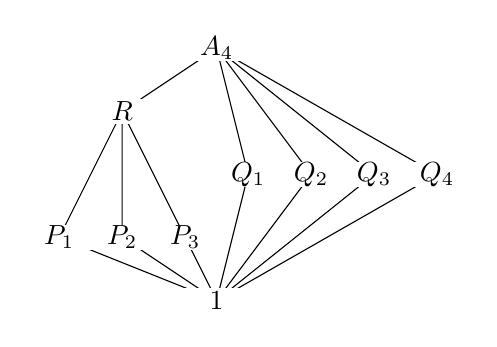
\begin{tikzpicture}[scale=0.8]
     \draw ( 0.0, 0) -- (-2.5, 1) -- (-1.5, 3);
     \draw ( 0.0, 0) -- (-1.5, 1) -- (-1.5, 3);
     \draw ( 0.0, 0) -- (-0.5, 1) -- (-1.5, 3);
     \draw ( 0.0, 0) -- ( 0.5, 2) -- ( 0.0, 4);
     \draw ( 0.0, 0) -- ( 1.5, 2) -- ( 0.0, 4);
     \draw ( 0.0, 0) -- ( 2.5, 2) -- ( 0.0, 4);
     \draw ( 0.0, 0) -- ( 3.5, 2) -- ( 0.0, 4);
     \draw (-1.5, 3) -- ( 0.0, 4);
     \fill[white] (-3,-0.2) rectangle (4,0.2);
     \fill[white] (-3, 0.8) rectangle (0,1.2);
     \fill[white] ( 0, 1.8) rectangle (4,2.2);
     \fill[white] (-3, 2.8) rectangle (0,3.2);
     \fill[white] (-3, 3.8) rectangle (4,4.2);
     \draw ( 0.0, 0) node{$1$};
     \draw (-2.5, 1) node{$P_1$};
     \draw (-1.5, 1) node{$P_2$};
     \draw (-0.5, 1) node{$P_3$};
     \draw ( 0.5, 2) node{$Q_1$};
     \draw ( 1.5, 2) node{$Q_2$};
     \draw ( 2.5, 2) node{$Q_3$};
     \draw ( 3.5, 2) node{$Q_4$};
     \draw (-1.5, 3) node{$R$};
     \draw ( 0.0, 4) node{$A_4$};
    \end{tikzpicture}
    \hspace{3em}
    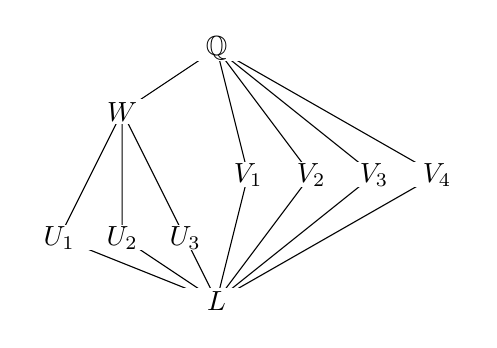
\begin{tikzpicture}[scale=0.8]
     \draw ( 0.0, 0) -- (-2.5, 1) -- (-1.5, 3);
     \draw ( 0.0, 0) -- (-1.5, 1) -- (-1.5, 3);
     \draw ( 0.0, 0) -- (-0.5, 1) -- (-1.5, 3);
     \draw ( 0.0, 0) -- ( 0.5, 2) -- ( 0.0, 4);
     \draw ( 0.0, 0) -- ( 1.5, 2) -- ( 0.0, 4);
     \draw ( 0.0, 0) -- ( 2.5, 2) -- ( 0.0, 4);
     \draw ( 0.0, 0) -- ( 3.5, 2) -- ( 0.0, 4);
     \draw (-1.5, 3) -- ( 0.0, 4);
     \fill[white] (-3,-0.2) rectangle (4,0.2);
     \fill[white] (-3, 0.8) rectangle (0,1.2);
     \fill[white] ( 0, 1.8) rectangle (4,2.2);
     \fill[white] (-3, 2.8) rectangle (0,3.2);
     \fill[white] (-3, 3.8) rectangle (4,4.2);
     \draw ( 0.0, 0) node{$L$};
     \draw (-2.5, 1) node{$U_1$};
     \draw (-1.5, 1) node{$U_2$};
     \draw (-0.5, 1) node{$U_3$};
     \draw ( 0.5, 2) node{$V_1$};
     \draw ( 1.5, 2) node{$V_2$};
     \draw ( 2.5, 2) node{$V_3$};
     \draw ( 3.5, 2) node{$V_4$};
     \draw (-1.5, 3) node{$W$};
     \draw ( 0.0, 4) node{$\Q$};
    \end{tikzpicture}
   \end{center}
   It follows that the lattice of subfields of $L$ is as shown on the
   right, where $U_i=L^{P_i}$ and $V_i=L^{Q_i}$ and $W=L^R$.  The
   larger subfields are towards the bottom, and the degrees are as
   follows: 
   \begin{align*}
    [L:U_i] &= 2 & [U_i:W] &= 2 & [W:\Q] &= 3 \\
    [L:V_i] &= 3 &         &    & [V_i:\Q] &= 4. 
   \end{align*}
   The field $W$ is normal over $\Q$, with $G(W/\Q)=A_4/R\simeq C_3$,
   but the fields $P_i$ and $Q_i$ are not normal over $\Q$.  \mks{4}
 \end{itemize}
\end{solution}

\end{document}
